\section{重心剖分}
\sourcepage{98--99}
本节证明，有限复形可以“剖分”为任意小的单形。单纯同调的讨论中要用到此结果，第四章讨论奇异同调时也要用到。

\entry{定义}{2.3.1}设 $K$ 为 $E^J$ 中的几何复形。若复形 $K'$ 满足以下条件，则称为 $K$ 的\textbf{剖分}（subdivision）：
\begin{enumerate}[label=(\arabic*)]
\item $K'$ 的每个单形包含在 $K$ 的某个单形中。
\item $K$ 的每个单形是 $K'$ 中有限多个单形的并。
\end{enumerate}
这些条件蕴含两复形的单形之并相同，即 $|K'|=|K|$ 作为集合相等。条件 (2) 的有限性还保证两者作为拓扑空间相同，容易验证。

若 $K''$ 为 $K'$ 的剖分，$K'$ 为 $K$ 的剖分，则 $K''$ 为 $K$ 的剖分。

若 $K_0$ 是 $K$ 的子复形，则 $K'$ 中所有位于 $|K_0|$ 的单形自动构成 $K_0$ 的剖分，称为\textbf{由 $K'$ 诱导的 $K_0$ 的剖分}。

下面的结果后文有用。

\entry{引理}{2.3.2}设 $K'$ 为 $K$ 的剖分。对于 $K'$ 的每个顶点 $w$，存在 $K$ 的顶点 $v$，使
\[
\operatorname{St}(w,K')\subset\operatorname{St}(v,K).\tag{$*$}
\]
事实上，若 $w\in\Int\sigma$，其中 $\sigma\in K$，则此包含关系成立，当且仅当 $v$ 是 $\sigma$ 的顶点。

\noindent\textbf{证明：}若 $(*)$ 成立，因为 $w\in\operatorname{St}(w,K')$，所以 $w$ 位于以 $v$ 为顶点的某个开单形中。

反过来，设 $w\in\Int\sigma$，$v$ 为 $\sigma$ 的顶点。只需证明
\[
|K|\setminus\operatorname{St}(v,K)\subset|K|\setminus\operatorname{St}(w,K').
\]
左边是 $K$ 中所有不以 $v$ 为顶点的单形之并，因此也是 $K'$ 的某些单形 $\tau$ 的并。这样的 $\tau$ 不可能以 $w$ 为顶点，因为 $w\in\Int\sigma\subset\operatorname{St}(v,K)$。所以每个这样的单形都位于右边。\hfill$\square$

\entry{例}{2.3.3}设 $K$ 由 $1$ 维单形 $[0,1]$ 及其顶点组成。设 $L$ 由各 $[1/(n+1),1/n]$（$n=1,2,\ldots$）、它们的顶点以及顶点 $0$ 组成。则 $|L|=|K|$ 作为集合相同，但作为拓扑空间不同。$L$ 满足剖分的所有条件，唯独不满足条件 (2) 的有限性。

\entry{例}{2.3.4}设 $\Sigma$ 由 $2$ 维单形 $\sigma$ 及其各面组成。图 2.3.1 中 $\Bd\sigma$ 的剖分 $K$ 可扩张为 $\Sigma$ 的剖分 $\Sigma'$：取内部点 $w$，作锥 $w*K$ 即可。称其为\textbf{从 $w$ 对 $K$ 作星形剖分}（starring $K$ from $w$）。这种方法后面很有用。
\begin{center}
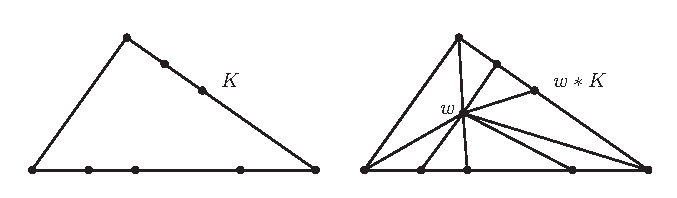
\includegraphics[width=117mm]{figures/2-3-1.pdf}\\图 2.3.1
\end{center}
下面描述一般复形的星形剖分方法，先需一个引理，证明留作习题。

\entry{引理}{2.3.5}复形 $K$ 的任意一族子复形的交仍为子复形。反过来，若 $\{K_\alpha\}$ 为 $E^J$ 中的一族复形，每一对底空间的交 $|K_\alpha|\cap|K_\beta|$ 都是同时为两者子复形的某个复形的多胞体，则并 $\bigcup_\alpha K_\alpha$ 为复形。

构造剖分采用逐步进行的方法，下面描述其中一步。

\entry{定义}{2.3.6}设 $L_p$ 是 $K$ 的 $p$ 维骨架的剖分。对于 $K$ 的 $(p+1)$ 维单形 $\sigma$，$\Bd\sigma$ 是 $p$ 维骨架的某个子复形的多胞体，因此也是 $L_p$ 的某个子复形的多胞体，以 $L_\sigma$ 表示后者。若 $w_\sigma\in\Int\sigma$，则锥 $w_\sigma*L_\sigma$ 的底空间为 $\sigma$。令 $L_{p+1}$ 为 $L_p$ 与所有这些锥的并。下面说明它是复形，称为\textbf{从各点 $w_\sigma$ 对 $L_p$ 作星形剖分而得到的 $K^{(p+1)}$ 的剖分}。

事实上，$|w_\sigma*L_\sigma|\cap|L_p|=\Bd\sigma$，它是同时为锥和 $L_p$ 的子复形 $L_\sigma$ 的多胞体。\translatornote{原文此处有 $W_p,W_\sigma,L_p$ 等下标、字母误印；这里按前述定义统一为 $w_\sigma,L_\sigma$。}若 $\tau$ 为另一个 $(p+1)$ 维单形，则两个锥的底空间相交于 $\sigma\cap\tau$，它是 $L_p$ 的某个子复形的多胞体，因此也同时对应 $L_\sigma,L_\tau$ 的子复形。由引理，$L_{p+1}$ 为复形。

\sourcepage{100--101}
$L_{p+1}$ 依赖各点 $w_\sigma$ 的选择。常取单形的典范内点，通常如下。

\entry{定义}{2.3.7}若 $\sigma=v_0\cdots v_p$，定义其\textbf{重心}（barycenter）为
\[
\widehat\sigma=\frac1{p+1}\sum_{i=0}^p v_i.
\]
这是关于各顶点的重心坐标都相等的内点。若 $\sigma$ 为边，$\widehat\sigma$ 为其中点；若为顶点，则 $\widehat\sigma=\sigma$。一般地，它也是 $\sigma$ 的质心，但本书不使用此事实。

\entry{定义}{2.3.8}设 $K$ 为复形，逐步定义其骨架的剖分。令 $L_0=K^{(0)}$。若 $L_p$ 已为 $p$ 维骨架的剖分，则从 $K$ 中各 $(p+1)$ 维单形的重心对 $L_p$ 作星形剖分，得到 $L_{p+1}$。由引理 2.3.5，各 $L_p$ 的并为 $K$ 的一个剖分，称为\textbf{第一次重心剖分}（first barycentric subdivision），记作 $\operatorname{sd}K$。

再对它作第一次重心剖分，得到 $\operatorname{sd}(\operatorname{sd}K)$，记为 $\operatorname{sd}^2K$，称为第二次重心剖分。类似定义任意正整数次剖分 $\operatorname{sd}^nK$。

有时需要明确描述第一次重心剖分的单形。用 $\sigma_1\succ\sigma_2$ 表示“$\sigma_2$ 为 $\sigma_1$ 的真面”。

\entry{引理}{2.3.9}$\operatorname{sd}K$ 恰由所有形如 $\widehat\sigma_1\widehat\sigma_2\cdots\widehat\sigma_n$ 的单形组成，其中 $\sigma_1\succ\sigma_2\succ\cdots\succ\sigma_n$。

\noindent\textbf{证明：}归纳。位于 $K^{(0)}$ 的剖分中的单形显然如此：它们是 $K$ 的顶点，且 $\widehat v=v$。假定结论对位于 $|K^{(p)}|$ 的单形成立。若 $\tau$ 位于 $|K^{(p+1)}|$ 而不位于 $|K^{(p)}|$，则它属于某个 $\widehat\sigma*L_\sigma$，其中 $\sigma$ 为 $(p+1)$ 维单形，$L_\sigma$ 为其真面复形的第一次重心剖分。由归纳假设，$L_\sigma$ 的单形形如 $\widehat\sigma_1\cdots\widehat\sigma_n$，其中各 $\sigma_i$ 都为 $\sigma$ 的真面，且依次为真面。因此 $\tau$ 形如 $\widehat\sigma\widehat\sigma_1\cdots\widehat\sigma_n$，正是所需形式。\hfill$\square$

\entry{例}{2.3.10}图 2.3.2 给出了复形 $K$ 及其前两次重心剖分。注意，第一次剖分的每个单形都有引理 2.3.9 的形式。还要注意，随着 $n$ 增大，$\operatorname{sd}^nK$ 的单形迅速变小。下面证明这是一般事实。
\begin{center}
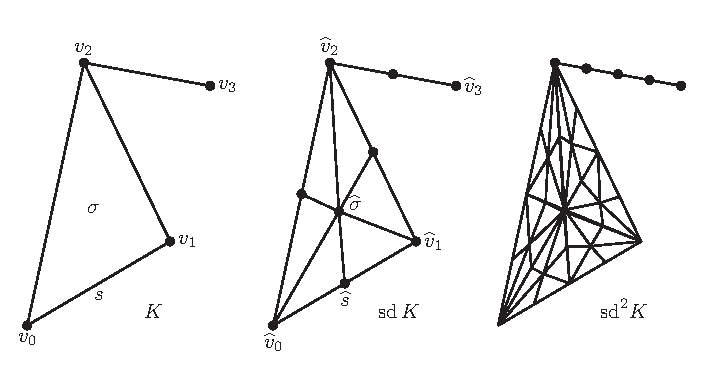
\includegraphics[width=122mm]{figures/2-3-2.pdf}\\图 2.3.2
\end{center}

\entry{定理}{2.3.11}给定有限复形 $K$、$|K|$ 的一个度量及 $\epsilon>0$，存在正整数 $N$，使 $\operatorname{sd}^NK$ 中每个单形的直径都小于 $\epsilon$。

\noindent\textbf{证明：}$K$ 有限，因此 $|K|$ 是其所在欧氏空间的子空间；又因为它紧致，选择哪个相容度量无关紧要。事实上，两个相容度量 $d_1,d_2$ 之间的恒等映射一致连续，给定 $\epsilon$，存在 $\delta>0$，使任何 $d_1$ 直径小于 $\delta$ 的集合，其 $d_2$ 直径小于 $\epsilon$。所以可用环境空间的度量
\[
|x-y|=\max_\alpha|x_\alpha-y_\alpha|.
\]
\textbf{第一步。}若 $\sigma=v_0\cdots v_p$，则其直径为顶点最大距离 $\ell=\max_{i,j}|v_i-v_j|$。显然 $\operatorname{diam}\sigma\geq\ell$，证明反向不等式。

先证对每个 $x\in\sigma$，$|x-v_i|\leq\ell$。以 $v_i$ 为中心、半径 $\ell$ 的闭邻域 $C(v_i;\ell)=\{x:|x-v_i|\leq\ell\}$ 是凸集，包含所有顶点，故包含 $\sigma$。

再固定 $x\in\sigma$。由刚才的结论，凸闭邻域 $C(x;\ell)$ 包含全部顶点，因此包含 $\sigma$。所以任意 $x,z\in\sigma$ 都满足 $|x-z|\leq\ell$，得到所需上界。

\sourcepage{102--103}
\textbf{第二步。}若 $\dim\sigma=p$，则每个 $z\in\sigma$ 满足
\[
|\widehat\sigma-z|\leq\frac p{p+1}\operatorname{diam}\sigma.
\]
计算
\[
\begin{aligned}
|v_0-\widehat\sigma|
&=\left|v_0-\sum_{i=0}^p\frac1{p+1}v_i\right|\\
&\leq\sum_{i=0}^p\frac1{p+1}|v_0-v_i|\\
&\leq\frac p{p+1}\max_i|v_0-v_i|
\leq\frac p{p+1}\operatorname{diam}\sigma.
\end{aligned}
\]
其他顶点也类似。因此以重心为中心、半径 $p\operatorname{diam}\sigma/(p+1)$ 的凸闭邻域包含全部顶点，故包含 $\sigma$。

\textbf{第三步。}若 $\sigma$ 为 $p$ 维单形，$\tau$ 为其第一次重心剖分的单形，则
\[
\operatorname{diam}\tau\leq\frac p{p+1}\operatorname{diam}\sigma.
\]
对维数归纳。$p=0$ 平凡。假定低于 $p$ 的维数成立。由引理 2.3.9 与第一步，只需对 $\sigma$ 的面 $s\succ s'$ 证明
\[
|\widehat s-\widehat{s'}|\leq\frac p{p+1}\operatorname{diam}\sigma.
\]
若 $s=\sigma$，由第二步得到。若 $s$ 为 $q$ 维真面，则
\[
|\widehat s-\widehat{s'}|\leq\frac q{q+1}\operatorname{diam}s
\leq\frac p{p+1}\operatorname{diam}\sigma.
\]
第一个不等式由归纳假设，第二个因为 $x/(x+1)$ 对 $x>0$ 递增。

\textbf{第四步。}设 $\dim K=n$，其单形最大直径为 $d$。第 $N$ 次重心剖分中单形的最大直径不超过 $(n/(n+1))^Nd$。\translatornote{原文将此表达式直接写为最大直径；前面证明给出的是上界，这已足够。}$N$ 足够大时，小于 $\epsilon$。\hfill$\square$

以下定义用于习题 2、3。

\entry{定义}{2.3.12}
\begin{enumerate}[label=(\arabic*)]
\item 对集合族 $\mathcal A,\mathcal B$，若每个 $B\in\mathcal B$ 都包含于某个 $A\in\mathcal A$，则称 $\mathcal B$ \textbf{加细} $\mathcal A$（refines）。
\item 若存在整数 $m$，使空间 $X$ 的每个开覆盖 $\mathcal A$ 都有一个开覆盖加细 $\mathcal B$，且 $X$ 中没有点属于 $\mathcal B$ 的多于 $m+1$ 个成员，则称 $X$ 具有\textbf{有限覆盖维数}。
\item 满足 (2) 的最小整数 $m$ 称为 $X$ 的\textbf{覆盖维数}（covering dimension）。
\end{enumerate}
习题 3 涉及 Cantor 三分集。为完整起见给出定义，得到的就是通常“不断去掉中间三分之一”的集合。

\entry{定义}{2.3.13}对每个正整数 $m$，令
\[
C_m=\bigcup_{k=0}^{(3^m-1)/2}\left[\frac{2k}{3^m},\frac{2k+1}{3^m}\right].
\]
\textbf{Cantor 三分集}定义为 $C=\bigcap_{m=1}^\infty C_m$。

\subsection*{习题}
\begin{enumerate}
\item 设 $K$ 为复形，$x_0\in|K|$。
\begin{enumerate}[label=(\alph*)]
\item 证明存在顶点集包含 $x_0$ 的剖分。
\item[\textasteriskcentered\,(b)] 证明存在顶点集恰由 $x_0$ 和 $K$ 的原有顶点组成的剖分。
\end{enumerate}
\item \begin{enumerate}[label=(\alph*)]
\item 证明离散集的覆盖维数为 $0$。
\item 证明 $[0,1]$ 的覆盖维数为 $1$。
\item 若 $X$ 的覆盖维数为 $m$，证明其任意闭子空间 $A$ 的覆盖维数至多为 $m$。
\item 若 $K$ 为 $m$ 维有限复形，证明 $|K|$ 的覆盖维数存在且至多为 $m$。［后面将看到它恰好为 $m$。］
\end{enumerate}
\item 计算 Cantor 三分集的覆盖维数。
\end{enumerate}
